\section{Numerical results}
\label{sec:results}

The operating point used throughout is
$k_xd=0.7362$, $k_yd=0.1298$, $\omega=7.6334\,c_s/d$, i.e.\
$f=\SI{16.68}{\giga\hertz}$ for $d=\SI{200}{\nano\metre}$, with the coupling
set to zero unless a sweep says otherwise, and with grounded faces.  The reference plane for each reported share is $L=10\,d=\SI{2}{\micro\metre}$ from
the edge.  Unless stated otherwise the Galerkin degree is $n=22$.

\subsection{Dispersion, wave speeds and the operating point}
\label{sec:results_dispersion}
\label{sec:results_scope}

\Cref{fig:fig01} characterizes the guided branch that is later scattered at the
edge.  Panel (a) plots the frequency against $k_xd$ for the five coupling
levels.  The five curves superimpose to within the width of the line over the entire range $0.15\le k_xd\le1.05$, and the inset resolves their difference: the
coupling lowers the frequency by at most \SI{184}{\kilo\hertz}, at
$k_xd=1.05$, where the frequency is \SI{16.87}{\giga\hertz}, that is by
$1.1\times10^{-5}$ in relative terms; at the negative coupling the lowering remains below \SI{92}{\kilo\hertz} over the same range.  This is the first indication, confirmed in \cref{sec:results_coupling},
that the added coupling is a perturbation of the dispersion and a modifier of the edge partition, and does not drive the branch.

Panel (b) shows three different velocities:
\begin{align}
v_p&=\frac{\omega}{|\vect{k}|}=\frac{\omega}{\sqrt{k_x^2+k_y^2}},
\qquad \text{(phase speed, a magnitude)}\label{eq:vp}\\
v_g&=c_s\frac{\partial\omega}{\partial k_x},
\qquad \text{(group velocity, signed)}\nonumber\\
v_E&=\frac{\mathcal{P}_x}{E},
\qquad \text{(energy velocity, signed)}\nonumber
\end{align}
with $\mathcal{P}_x$ from \eqref{eq:Px_int} and $E$ the stored energy per unit
length.  The phase speed \eqref{eq:vp} is a positive magnitude and cannot
change sign; it is plotted on the right-hand axis of panel (b) and it decreases
monotonically from \SI{105.8}{\kilo\metre\per\second} near the cutoff at
$k_xd=0.15$ to \SI{20.0}{\kilo\metre\per\second} at $k_xd=1.05$.  The
group and energy velocities are signed and are plotted on the left-hand axis:
they run from $-189$ and $-189$ to $+1136$ and $+1136\,\si{\metre\per\second}$,
change sign just below $k_xd=0.53$, and agree with each other to within
\SI{0.03}{\percent} at every sample; the group velocity is a symmetric difference of half-width $0.0025$ in $k_xd$.  The sign change of $v_g$ and $v_E$ marks the backward part of the branch.  A
backward branch exists whether or not an edge is present, and what the edge adds
is the conversion into it: the branch provides a mode whose energy travels
opposite to the phase, and that is the mode the edge subsequently selects.

Panels (c) and (d) report the linewidth and the attenuation.  The linewidth
ranges from \SI{1.4}{\kilo\hertz} to \SI{0.27}{\mega\hertz} and grows
monotonically with $k_xd$; it is smallest at $H=0$ and rises with $|H|$, further
for positive than for negative coupling.  The attenuation
$\alpha=2|\Imag k_x|$, obtained from the complex spatial root at real frequency and quoted in decibels of power as $4.343\,\alpha$,
ranges from \SI{0.11}{\deci\bel\per\milli\metre} to
\SI{228}{\deci\bel\per\milli\metre} and is positive everywhere on the branch.
It is largest on the slow part of the branch, but the plotted grid of
$\Delta k_xd=0.03$ resolves that maximum only at its own sample, $k_xd=0.54$:
the fold has \SIrange{43.5}{44.5}{\deci\bel\per\milli\metre} at $H=0$
(\cref{tab:configurations}), which a raster of that spacing cannot show.

\begin{figure}[htbp]
\centering
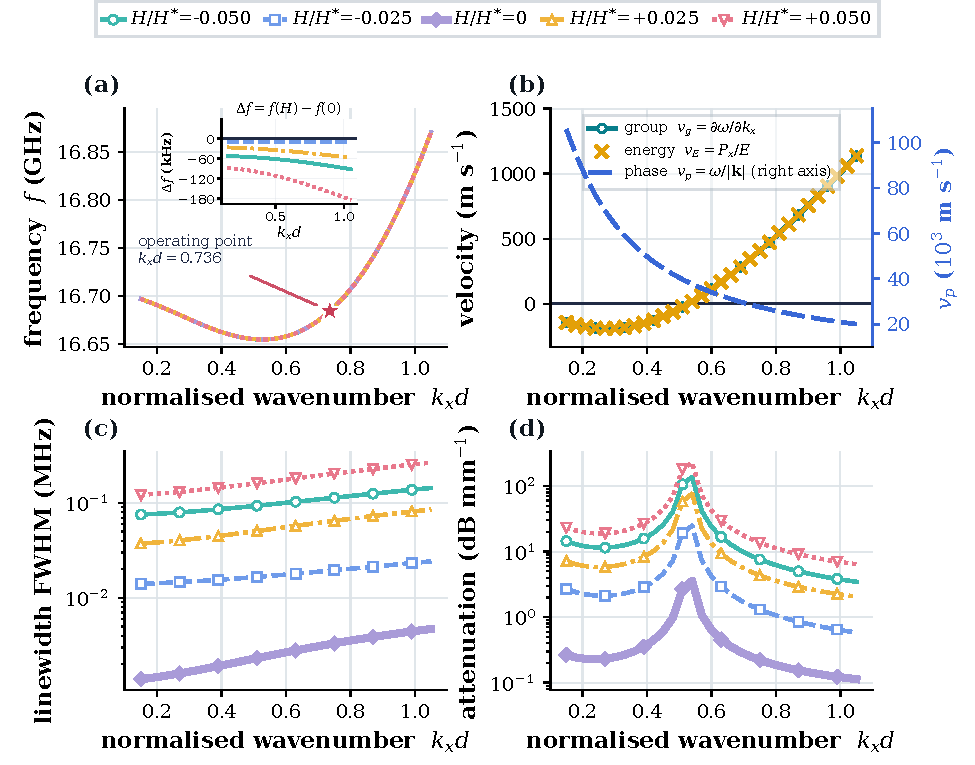
\includegraphics[width=0.95\textwidth]{figures/fig01_dispersion.pdf}
\caption{Guided branch at $k_yd=0.1298$, $d=\SI{200}{\nano\metre}$, $\ell=\SI{50}{\nano\metre}$. (a) Frequency against $k_xd$, with the inset showing $\Delta f=f(H)-f(0)$; the operating point $k_xd=0.736$ is marked. (b) Group, energy and phase speeds at $H=0$. (c) Linewidth and (d) attenuation, $4.343\times2|\Imag k_x|$ in dB mm$^{-1}$, for five coupling levels.}
\label{fig:fig01}
\end{figure}


Before the numbers are read, the part of \eqref{eq:enthalpy} exercised by the calculations should be stated.

Four sectors are active in each solve: the elastic, the strain-gradient, the
piezoelectric and the carrier sector.  The flexoelectric sector is active but
subdominant.  A single flexoelectric constant $f\equiv f_{3zz}=\SI{1}{\nano
\coulomb\per\metre}$ is retained.  It lies at the low end of the range
reported for ZnO \cite{hu2025computational,zhao2021effects} and is an assumed value, taken independently of the
crystal used for the elastic constants; it gives the dimensionless
coupling $f=2.56\times10^{-3}$ of \cref{tab:groups}.  The added
carrier--strain-gradient coupling is swept over
$|H|\le\SI{2.0e-23}{\joule\metre}=0.022\,H_{\text{bound}}$, i.e.\ over the
range allowed by \eqref{eq:schur}.

The flexoelectric term was tested directly, by repeating the two solved configurations with $f$ set to zero and to ten times
the retained value.  At the
operating point the backward
channel is $0.0192916$ with the retained $f$ and $0.0192938$ with $f=0$, a
change of \SI{-0.012}{\percent}; at $k_xd=0.55$ it is $0.551910$ and
$0.551976$, a change of \SI{-0.012}{\percent}.  At ten times the retained value the changes
are \SI{-1.16}{\percent} and \SI{-1.18}{\percent}, so the dependence is smooth
and quadratic in the coupling (a factor of 97 for a factor of ten), with no threshold.

Taken together, these numbers place the reported shares within one part in ten
thousand of the shares of the \emph{strain-gradient
piezoelectric-semiconductor} specialization with the added carrier coupling.
The flexoelectric term is present and contributes with the correct sign and
magnitude, and it does not drive the effect.  What the numbers support is a
slow-mode edge effect of the strain-gradient plate, modulated by the carrier
coupling, inside a flexoelectric-semiconductor formulation; they do not support
the attribution of the negative reflection to the flexoelectric mechanism
itself.

\subsection{Dependence on carrier density, thickness and frequency}
\label{sec:results_material}
\label{sec:results_geometry}
\label{sec:results_frequency}

\Cref{fig:fig02} sweeps the two material families.  Increasing the carrier
density from $1$ to $3\times10^{18}\,\si{\per\cubic\metre}$ raises the linewidth
(a) and the attenuation (b) by a factor of three each (the conduction loss is
linear in the density over this range) and lowers the frequency only
slightly.  Panel (c) is the most informative: the backward channel at the reference plane is plotted against
$k_xd$ for the five densities, and the five curves collapse onto one.  The
largest sampled value, $R_B\approx0.552$ ($0.5515$ to $0.5523$), is at $k_xd=0.55$ for all densities; this raster of $\Delta k_xd=0.05$ does not resolve the fold at $k_xd=0.527$, whose maximum is given in \cref{sec:results_peak}.  The
relative spread between the five curves is below \SI{0.2}{\percent} over the full range.  On this raster, and over this factor-of-three range, the carrier density thus sets the loss but not the partition of the scattered power (see \cref{sec:results_sens} for a wider range).

The mobility behaves in the same way (panel d): over the factor-of-three range
$0.00875$ to $0.02625\,\si{\square\metre\per\volt\per\second}$ the linewidth
changes by the same factor of three, while the backward share is unchanged to
the same $0.2$ percent.  The two sweeps agree row by row because both quantities enter the conduction
term through their product, while the density also enters the screening through
$Q^{2}=5.6\times10^{-3}$, which is small here; the two are therefore equivalent at this $Q$ and not interchangeable in
general (see \cref{sec:results_sens} for larger densities).  Both results are consistent with $Q=d/L_D=0.075<1$: the
plate is thinner than the Debye length, the carrier perturbation is not confined
to a surface layer, and the density enters the problem mainly through the
conduction loss.

Every row of this sweep satisfies the conservation bound \eqref{eq:admissible}; the curve in panel (c) extends to $k_xd=0.9$, falling below
$10^{-7}$ beyond $k_xd=0.8$ and reaching between $3\times10^{-12}$ and $1\times10^{-11}$ at the last sample.  This is the backward port ceasing to carry energy, not a numerical failure.  Rows at that end have $|\cos\theta_E|\to0$, and the flux
fraction is evaluated at each point so that the loss of resolution is visible.

\begin{figure}[htbp]
\centering
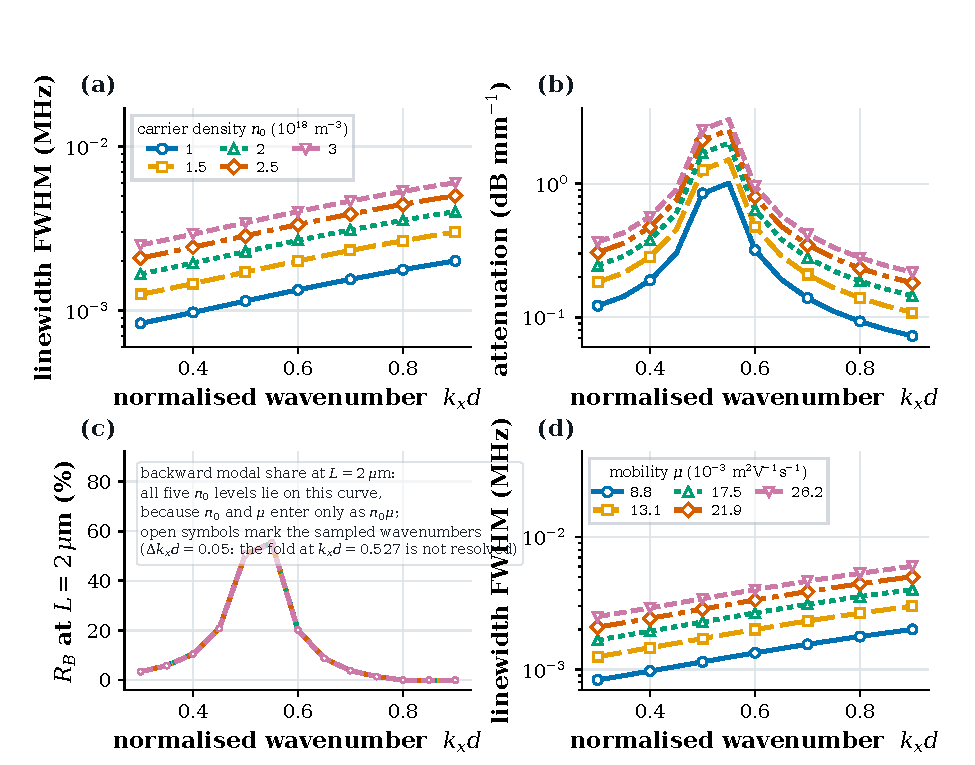
\includegraphics[width=0.95\textwidth]{figures/fig02_material.pdf}
\caption{Carrier density and mobility at $H=0$, $k_yd=0.1298$, sampled every $\Delta k_xd=0.05$. (a) Linewidth and (b) attenuation ($4.343\times2|\Imag k_x|$) for five $n_0$; (c) backward share at $L=\SI{2}{\micro\metre}$; (d) linewidth for five mobilities.}
\label{fig:fig02}
\end{figure}


\Cref{fig:fig03} separates the two geometric families, which scale differently
and must not be plotted on a common axis.  Plate thickness is the dominant
scale: across the family between \SI{120}{\nano\metre} and \SI{320}{\nano\metre}
the branch lies between \SI{10.5}{\giga\hertz} and \SI{30.4}{\giga\hertz}, and
the relative change is of order unity at all wavenumbers (panels a and c).  The gradient length shifts the same
branch by a smaller amount than the thickness (panels b and d): relative to
$\ell=\SI{50}{\nano\metre}$, a change to $\ell=\SI{90}{\nano\metre}$ shifts the
frequency by \SI{+2.0}{\percent} at $k_xd=0.145$ and by \SI{+10.2}{\percent} at
$k_xd=1.00$, while $\ell=\SI{35}{\nano\metre}$ shifts it by \SI{-1.9}{\percent}
and \SI{-4.9}{\percent} at the same two points.  The sign of the effect changes
with $\ell$ across the reference value, so the panel is plotted as a
relative change and not as an absolute frequency.

The distinction matters for the interpretation of the rest of the paper.  A
thickness change rescales the whole problem and is not a coupling effect; a
gradient-length change alters the relative weight of the hyperelastic and
flexoelectric terms at fixed geometry and so is the parameter that belongs with $H$ in a discussion of the added physics.

\begin{figure}[htbp]
\centering
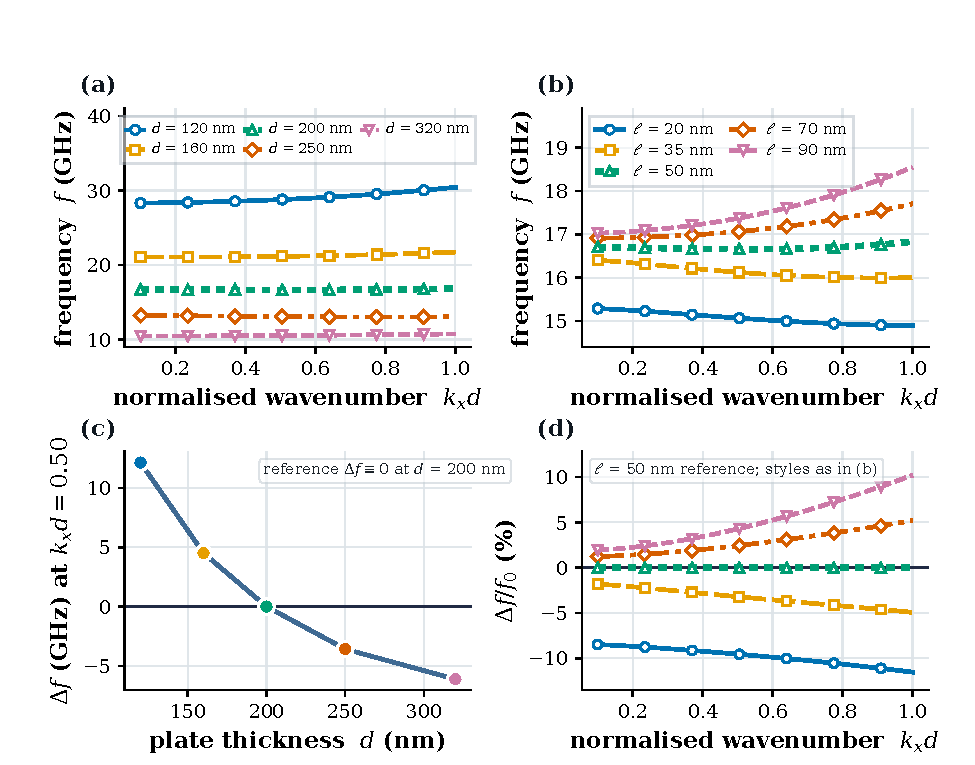
\includegraphics[width=0.95\textwidth]{figures/fig03_geometry.pdf}
\caption{Thickness and gradient length at $H=0$, $k_yd=0.1298$. (a) Dispersion for five thicknesses ($\ell=\SI{50}{\nano\metre}$); (b) dispersion for five gradient lengths ($d=\SI{200}{\nano\metre}$), each the operating-point branch followed from $\ell=\SI{50}{\nano\metre}$; (c) $\Delta f$ at $k_xd=0.50$ against thickness; (d) relative frequency change for five gradient lengths.}
\label{fig:fig03}
\end{figure}


\Cref{fig:fig04} sweeps the drive along the solved guided branch, not at a fixed frequency.  This matters away from the operating point, where
a fixed-frequency solve does not return the physical continuation of the branch
and the energy angle collapses towards $-90^{\circ}$; following the branch gives,
for each row, a resolved triple of frequency, wavenumber and share.  Two
rasters are used: a coarse one over the full window and, at $H=0$ only, a fine
one of spacing $\Delta k_xd=5\times10^{-4}$ across $0.520\le k_xd\le0.535$,
because the top of the response is three orders of magnitude narrower than any
raster that can be drawn on a single axis.  The number of rows is a property of
the grid.

The share along the branch is largest on its slow part.  It is $0.0341$
at $k_xd=0.30$ ($f=\SI{16.676}{\giga\hertz}$), rises to $0.9429$ at
$k_xd=0.52719$ ($f=\SI{16.6547}{\giga\hertz}$), and falls to $0.0142$ at
$k_xd=0.75$ ($f=\SI{16.688}{\giga\hertz}$) (panel a).  The response has a single peak over the entire window: the coarse raster finds no second local
extremum, and the top of the peak is located by a refined search.  Panel (b) shows the signed energy angle
changing by $17^{\circ}$ across the window and passing through its own extremum
next to the maximum of $R_B$, so the two are not independent readings.  Panel (c)
plots the same data against the ratio $k_{Bx}/k_{ix}$: all five coupling levels
collapse onto one master curve, and the conversion is largest where the backward
wavenumber approaches the incident one, reaching $k_{Bx}/k_{ix}=0.9960$ at the
maximum.  The backward port is a propagating mode on the
backward-slope part of the same branch, not an evanescent artifact, and the projection onto it
becomes decisive where the two wavenumbers approach each other.  Panel
(d) shows why they do: the branch passes through a zero-group-velocity point at
$k_xd\approx0.527$, where $|v_g|$ falls below \SI{1}{\metre\per\second} against
$-187$ and $+409\,\si{\metre\per\second}$ at the two ends of the window, and the
incident and backward wavenumbers close on one another there and open again
beyond it.

\begin{figure}[htbp]
\centering
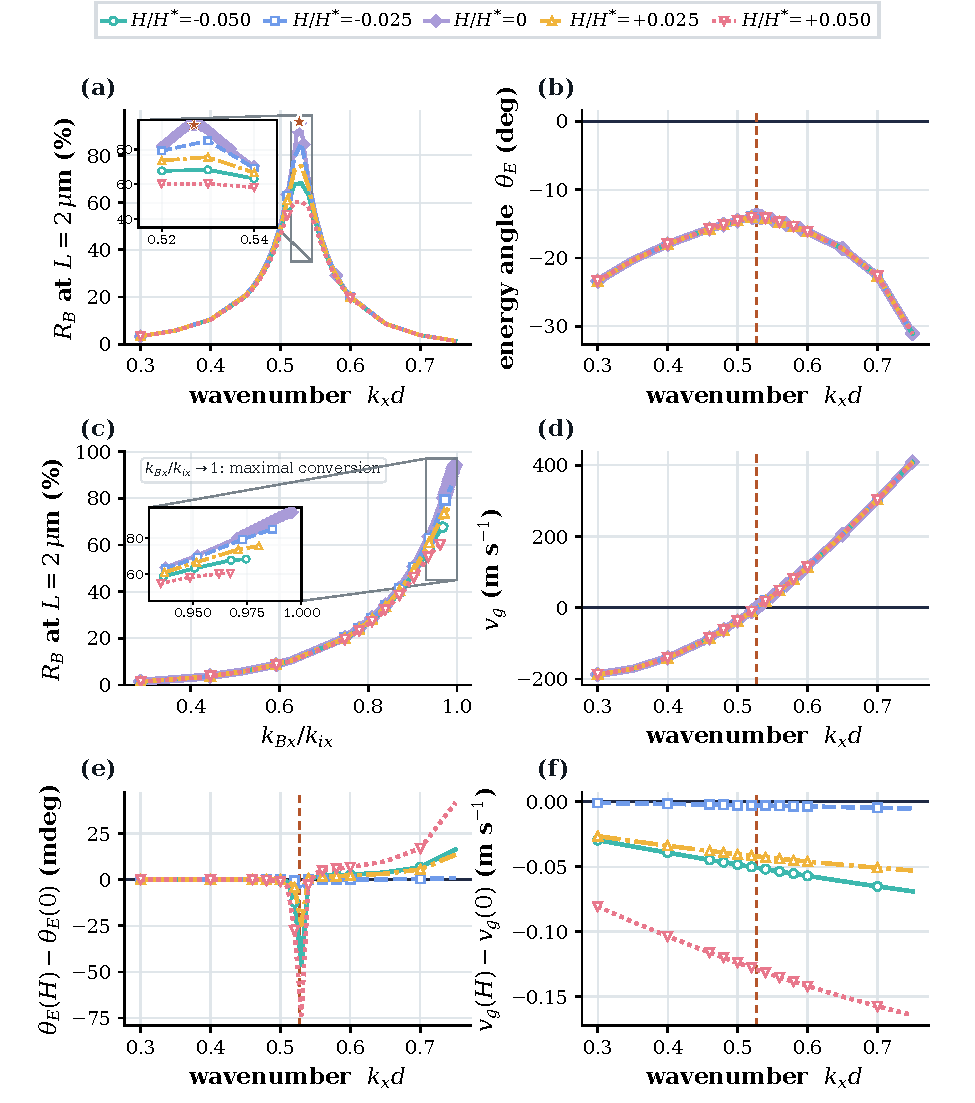
\includegraphics[width=0.95\textwidth]{figures/fig04_frequency.pdf}
\caption{Backward conversion along the branch at $k_yd=0.1298$, $L=\SI{2}{\micro\metre}$, with the frequency following the branch. (a) $R_B$ against $k_xd$, maximum marked by a star. (b) Energy angle. (c) $R_B$ against $k_{Bx}/k_{ix}$. (d) Group velocity. Insets magnify the region near the maximum; (e), (f) show the departure of (b) and (d) from $H=0$.}
\label{fig:fig04}
\end{figure}

In \cref{fig:fig04} the five coupling levels separate only near the maximum
(insets of panels a and c); the curves of panels (b) and (d) coincide on the
scale of the full response.  Panels (e) and (f) show that the energy angle
changes by at most $7\times10^{-2}$ degree, at the maximum, and the group
velocity by less than $0.2\,\si{\metre\per\second}$.  Every plotted row satisfies
the conservation bound \eqref{eq:admissible}.

\subsection{The branch maximum}
\label{sec:results_peak}
\label{sec:results_certification}

The maximum of \cref{fig:fig04} falls between two samples of the coarse raster, so it was solved again at six Galerkin degrees, each value being checked against the quadrature rule.  At degree $30$ the share is $0.019\,292$ at the operating point and $0.942\,872$ at the maximum.  Between degrees $14$ and $34$ the relative change of the maximum stays below $10^{-5}$ and that of the operating point is $2.5\times10^{-5}$, the successive changes decreasing monotonically; with the degree fixed at 22 and the rule taken from 64 to 256 nodes the maximum changes by less than $10^{-8}$.  The edge system is well conditioned (condition number at most $1.9\times10^{2}$, scaled edge residual below $3\times10^{-15}$), and the values are resolved projections: the energy angles are $-13.9^{\circ}$ and $-27.9^{\circ}$, so the measured $x$ flux is \SI{97.1}{\percent} and \SI{88.4}{\percent} of the total modal flux and neither value is an artifact of a near-grazing mode.

The quantity maximized is the one defined by \eqref{eq:RB}: the modal self-power of the identified backward outgoing mode at the reference plane, divided by the incident power at the same plane.  The other outgoing modes, the interference term and the dissipation are quoted separately and never folded into it.  A coarse raster of $\Delta k_xd=0.002$ over $0.465\le k_xd\le0.625$ (the whole window in which a backward port exists at this $k_y$) contains a single peak with its largest sample at $k_xd=0.527$, and a plateau raster of $10^{-4}$ and a refined raster of $10^{-5}$ place the maximum at $k_xd=0.52719$ with $R_B=0.9428718$.  The top is flat: every sampled wavenumber in $0.5267\le k_xd\le0.5276$ lies within \SI{0.01}{} percentage point of the maximum, so the reported location is the center of that top, determined to within $\pm0.0005$.  The incident wavenumber returned by the spatial problem is $k_{ix}d=0.52821$, \SI{0.19}{\percent} from the branch parameter, and no conclusion depends on the difference.  The result is a \emph{local maximum within the declared window}, not a global maximum over all $k_y$, thicknesses or material sets, none of which is searched here.

The maximum has a simple reading.  At the fold the group velocity vanishes ($+0.01\,\si{\metre\per\second}$ against $-187$ and $+409\,\si{\metre\per\second}$ at the ends of the solved window) and the backward and incident wavenumbers differ by \SI{0.4}{\percent}, so the two modes are nearly parallel and the edge conditions can be met with only a small admixture of the other outgoing modes; the projection onto the backward mode then takes almost all of the partition.  Panel (c) of \cref{fig:fig04} shows this: all coupling levels collapse onto one curve in $k_{Bx}/k_{ix}$, with the conversion maximal as the ratio approaches unity, and the conversion falls steeply on both flanks.  A grid of $\Delta k_xd=0.05$ would miss the maximum because the whole top of the response is $10^{-3}$ wide.  The same fold makes the incident flux fall by a factor of $131$ with respect to the operating point, so the partition is maximal where the transported power is minimal: that ninety-four percent of the energy is turned around would be true as a ratio and false as an energy budget, and only the ratio is claimed.  The outgoing propagating modes carry all of the incident power to within \SI{0.1}{\percent} (\cref{sec:results_channel}), so the plate is an almost perfect scatterer and the question is into which branch the power goes.  A measurement of the total reflectance would see essentially unity everywhere on the branch; the negative reflection requires modal resolution, by a wavenumber filter or a time-of-flight separation of the branches.

\subsection{Modal share and energy budget at the maximum}
\label{sec:results_artefact}
\label{sec:results_channel}

Three properties of the solution decide whether such a number can be read at
face value.

The incident flux at the maximum is small, a
factor $131$ below its value at the operating point, so the fraction could in
principle be a ratio of two nearly vanishing quantities.  It is not: the value
is reproduced to better than $10^{-5}$ across six Galerkin degrees, to
better than $10^{-8}$ across four quadrature rules, and to $2.3\times10^{-7}$ along three
different tracking paths that reach the same wavenumber from below, from above
and in a single step.  A ratio of two independently vanishing numbers would
scatter under all three.

The reference plane is moved from $0$ to $20$
thicknesses and the partition is rescaled by
$\exp[2(|\Imag k_{ix}|+|\Imag k_{Bx}|)(L-L_{\text{ref}})/d]$, which is the net
attenuation of the two partner modes travelling in opposite directions.  The
rescaled values agree to $2\times10^{-16}$, so the number is a property of the
edge and both attenuations are resolved and not assumed.  The transform is
applied identically to every result, and the edge-plane
fractions of the search, of the matched controls and of the coupling study
are reproduced by an independent re-evaluation to $10^{-10}$ relative or better; the plane at
which a share is quoted is hence a reporting choice and not a second
definition.  The backward port
is also unique: the second outgoing candidate lies $2.0|k_x|$ away, the
condition number of the normalized edge matrix is $1.4\times10^{2}$, and the
relative error bound of the projection is $\text{cond}\times\epsilon=4\times10^{-14}$.

The incident and backward eigenvectors
are nearly parallel, with overlap $0.999995$, and their wavenumbers are
separated by $1.45$ times the modal decay rate: close, but resolved.  The share also varies smoothly through the fold, taking the values $0.942\,777$, $0.942\,869$, $0.942\,872$, $0.942\,866$ and $0.942\,818$ at $k_xd=0.5267$, $0.5270$, $0.52719$, $0.5274$ and $0.5276$ at degree $22$, while the relative separation of the two wavenumbers stays within $0.2$ percent of its value at the maximum.  The
partition rebuilt from the amplitudes and modal powers alone reproduces the computed value to machine precision, which is the direct statement that no
eigenvector phase or scale enters the result.  What the near-coincidence does
change is interpretation, not accuracy: because the incident flux falls towards
the fold, the fraction is anti-correlated with it across the window, so a maximal share goes together with a minimal transported power.

The maximum is a modal share and not a reflectance.  At $k_xd=0.52719$ the
total outgoing propagating power is $1.00050$ of the incident power and the
interference correction at the reference plane is $+5.2\times10^{-4}$, so the
backward mode carries \SI{94.29}{\percent} of the incident power and
\SI{94.24}{\percent} of the outgoing propagating power.  At this fold the
interference term is sensitive at the level of $10^{-3}$ to the wavenumber at which the
frequency is fixed (it is $-8.0\times10^{-4}$ at the neighboring sample $k_xd=0.5275$, which has the same frequency to $10^{-8}$), whereas the modal share changes by $2\times10^{-5}$ relative.  The modal share is
\SI{94.29}{\percent}; the energy statement is that the propagating outgoing
modes carry the incident power to within \SI{0.1}{\percent}.  The two are different readings of the same
solution.

The maximum must also be read with its own amplitude in mind.  It lies on a zero-group-velocity fold, and a mode with vanishing group velocity carries
vanishing flux: the incident modal power per unit normalization falls from
$5.08\times10^{-3}$ at the operating point to $3.87\times10^{-5}$ at the
maximum, a factor $131$, while $|\Imag k_{ix}|d$ rises to $1.0\times10^{-3}$.
The fraction is the ratio of two small but resolved fluxes (well
defined, unchanged by the incident normalization, and stable to
$1\times10^{-5}$ under degree and quadrature refinement), but it is not a statement that a
large amount of energy is turned around.  Both readings are needed: the
partition is maximal at the fold and the transported power is minimal there.

The three configurations are compared term by term in
\cref{tab:configurations}.  Every entry is evaluated at degree 30, except the
attenuations, which are $2|\Imag k_x|/d$ formed from the same spatial roots and quoted in decibels of power ($4.343\times$).

\begin{table}[t]
\centering
\caption{The three reported configurations ($d=\SI{200}{\nano\metre}$, $\ell=\SI{50}{\nano\metre}$, $H=0$, $k_yd=0.1298$, $L=10d$). $R_B$ is a modal share, not a reflectance.}
\label{tab:configurations}
\scriptsize
\begin{tabular}{@{}lccc@{}}
\toprule
Quantity & Operating point & Maximum & $k_xd=0.55$ \\
\midrule
frequency & $\SI{16.684}{\giga\hertz}$ & $\SI{16.6547}{\giga\hertz}$ & $\SI{16.6550}{\giga\hertz}$ \\
longitudinal wavenumber $k_xd$ & 0.7362 & 0.52719 & 0.5500 \\
incident wavenumber $\Real k_{ix}d$ & 0.7362 & 0.5282 & 0.5500 \\
group velocity $v_g$ & $\SI{379}{\metre\per\second}$ & $\SI{0.01}{\metre\per\second}$ & $\SI{34}{\metre\per\second}$ \\
incident attenuation, $4.343\times2|\Imag k_{ix}|$ & \SI{0.235}{\deci\bel\per\milli\metre} & \SIrange{43.5}{44.5}{\deci\bel\per\milli\metre} & \SI{2.01}{\deci\bel\per\milli\metre} \\
backward attenuation, $4.343\times2|\Imag k_{Bx}|$ & \SI{0.227}{\deci\bel\per\milli\metre} & \SIrange{43.5}{44.5}{\deci\bel\per\milli\metre} & \SI{1.96}{\deci\bel\per\milli\metre} \\
backward share $R_B$ & $0.0192916$ & $0.9428718$ & $0.5519095$ \\
modal share at the edge plane & $0.0193$ & $0.9824$ & $0.5529$ \\
energy angle $\theta_E$ & $-27.90^{\circ}$ & $-13.85^{\circ}$ & $-14.45^{\circ}$ \\
total outgoing propagating power & $0.99980$ & $1.00050$ & $0.99878$ \\
interference $P_{\text{cross}}/P_{\text{inc}}$ & $-4.6\times10^{-6}$ & $+5.2\times10^{-4}$ & $-1.03\times10^{-3}$ \\
dissipation $P_{\text{diss}}/P_{\text{inc}}$ & $1.99\times10^{-4}$ & $2.78\times10^{-5}$ & $1.93\times10^{-4}$ \\
edge-system condition number & $\le 2\times10^{2}$ & $\le 2\times10^{2}$ & $\le 2\times10^{2}$ \\
scaled edge residual & $\le3\times10^{-15}$ & $\le3\times10^{-15}$ & $\le3\times10^{-15}$ \\
\bottomrule
\end{tabular}
\end{table}


\Cref{fig:fig05} closes the energy identity \eqref{eq:energy_identity} at the
reference plane.  At $H=0$ the incident power normalized to unity is partitioned
as follows: the identified backward channel carries $1.9292\times10^{-2}$, the
remaining propagating outgoing modes carry $0.980505$, dissipation removes
$1.989\times10^{-4}$, and the interference term is $-4.6\times10^{-6}$.  The
first two sum to $0.999796$, the total outgoing propagating power; adding the
dissipation leaves $5\times10^{-6}$ of the incident power, which is the magnitude of the interference term to the six digits quoted.  The
interference term is defined as the remainder of the identity, so the sum closes
by construction; the independent check is the balance of the flux at the
reference plane against the edge flux and the conduction loss, which closes to
better than $10^{-11}$ relative at each Galerkin degree from 14 to 34, five
orders of magnitude below the $10^{-6}$ threshold plotted in panel (c).  At the maximum
the backward channel carries $0.942872$ and the remaining propagating modes
$5.76\times10^{-2}$, which together account for $1.00050$ of the incident
power; dissipation removes $2.78\times10^{-5}$ and the interference term is
$+5.2\times10^{-4}$.  The same power balance closes there to
$6\times10^{-14}$.

The evanescent spectrum does not belong to the transported budget.  At the
reference plane the entire evanescent content has decayed by a factor
$\exp(-2|{\Imag k_x}|L)$ with $|{\Imag k_x}|L\gtrsim10$, which leaves
$4.8\times10^{-28}$ of the incident power.  Reactive accounting is meaningful
only at the edge plane, where it is $4.4\times10^{-6}$, and even there it
is not transported energy.  For the same reason $P_{\text{cross}}$ is an
interference correction and not a channel, and the evanescent members of
$\{P_j\}$ are reactive; the complete statement is the partition above, with the
interference term quoted explicitly.

Panels (b) and (d) sweep the coupling at the \emph{fixed} operating frequency
$\omega=\omega_0$, so the incident wavenumber drifts with $H$ along the branch
instead of the frequency doing so.  That is the response of the plate driven at
one frequency; the branch-consistent comparison is the relevant one.  At
fixed frequency the backward channel changes from $1.9051\times10^{-2}$ at
$H/H^{*}=-0.05$ to $1.8876\times10^{-2}$ at $H/H^{*}=+0.05$, a variation of
\SI{0.92}{\percent}; dissipation rises from $6.9\times10^{-3}$ to
$1.2\times10^{-2}$; the other propagating modes carry the balance.  Panel (d)
gives the same information as a relative change against the uncoupled baseline:
the largest deviation is \SI{-2.15}{\percent} at $H/H^{*}=+0.05$.  When instead
$k_x$ is held fixed and the frequency follows the branch (the branch-consistent comparison), the deviation at the same tabulated extreme is
\SI{-1.21}{\percent}: part of the fixed-frequency variation is the dispersion
shift of $H$, which reaches $6.3\times10^{-5}$ in $\omega$.

\begin{figure}[htbp]
\centering
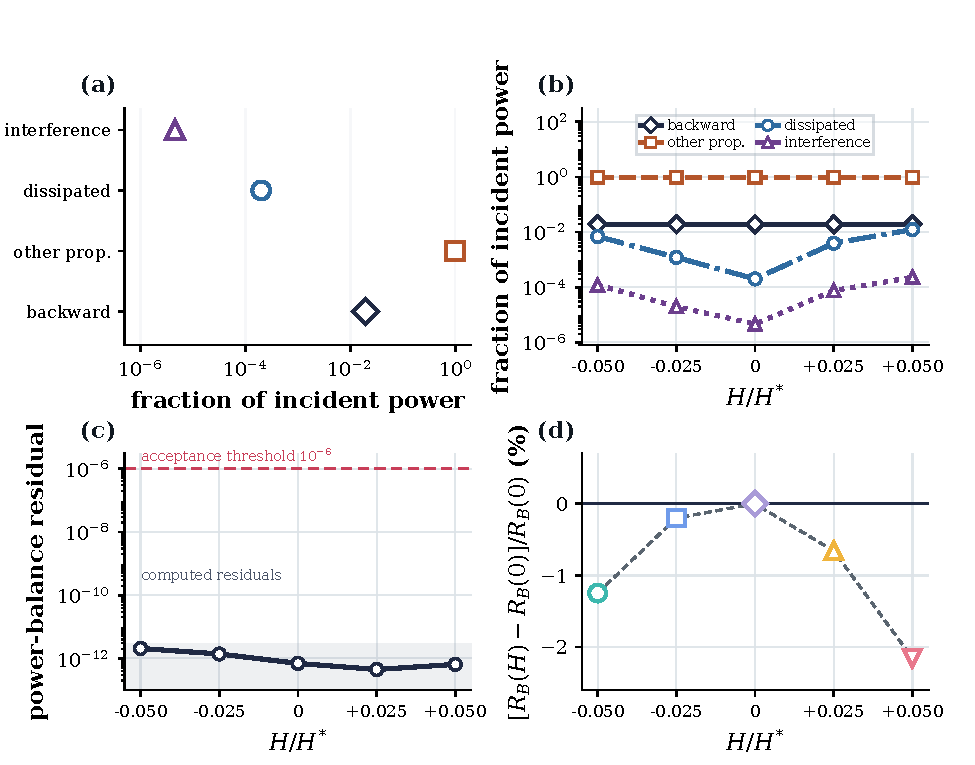
\includegraphics[width=0.95\textwidth]{figures/fig05_channel.pdf}
\caption{Energy budget at the operating point and the reference plane $x=-10\,d$; the interference term is shown as a magnitude. (a) Partition at $H=0$. (b) The same fractions against $H/H^{*}$ at fixed frequency. (c) Power-balance residual. (d) Relative change of the backward channel.}
\label{fig:fig05}
\end{figure}

\subsection{The backward channel}
\label{sec:results_mechanism}
\label{sec:results_attenuation}

The partition quoted above was computed at $H=0$, with the
carrier--strain-gradient coupling switched off, and the contribution of that
coupling is isolated by matched controls: each ingredient except the named one
is held fixed (same $k_x$, same $k_y$, same $n_0$, same $\ell$, same reference
plane, same unit incident self-power), and the frequency follows the branch,
because switching an ingredient off changes the dispersion and solutions taken at
different frequencies of a different branch would not be comparable.
\Cref{tab:controls} lists the outcome.

\begin{table}[t]
\centering
\caption{Matched controls. The frequency follows the branch. Entries marked ``sp'' are specular self-powers, not backward conversion.}
\label{tab:controls}
\footnotesize
\begin{tabularx}{\textwidth}{@{}>{\raggedright\arraybackslash}Xcccccc@{}}
\toprule
 & \multicolumn{2}{c}{Operating point ($k_xd=0.736$)}
 & \multicolumn{2}{c}{Maximum ($k_xd=0.52719$)}
 & \multicolumn{2}{c}{$k_xd=0.550$} \\
\cmidrule(lr){2-3}\cmidrule(lr){4-5}\cmidrule(lr){6-7}
Configuration & freq.\ (GHz) & $R_B$ & freq.\ (GHz) & $R_B$ & freq.\ (GHz) & $R_B$ \\
\midrule
full ($f_0$, $H/H^{*}=+0.05$) & 16.6840 & 0.019\,058 & 16.6546 & 0.602\,292 & 16.6549 & 0.495\,776 \\
$f=f_0$, $H=0$                & 16.6841 & 0.019\,292 & 16.6547 & 0.942\,872 & 16.6550 & 0.551\,910 \\
$f=0$, $H/H^{*}=+0.05$        & 16.6840 & 0.019\,060 & 16.6546 & 0.602\,290 & 16.6549 & 0.495\,822 \\
$f=0$, $H=0$                  & 16.6841 & 0.019\,294 & 16.6547 & 0.942\,878 & 16.6550 & 0.551\,976 \\
$\ell=0$, $f=0$, $H=0$        & 16.2077 & 0.075\,961$^{\mathrm{sp}}$
                              & 15.9717 & 0.133\,278$^{\mathrm{sp}}$
                              & 15.9943 & 0.124\,109$^{\mathrm{sp}}$ \\
\bottomrule
\end{tabularx}
\end{table}

Three statements follow.

First, the effect is already present with $H=0$: the same branch converts
\SI{1.93}{\percent} at the operating point and \SI{94.29}{\percent} at the
maximum.  The strain-gradient piezoelectric-semiconductor model already contains the partition, and the coupling can only modify it.

Second, the size of the modification depends strongly on where the branch is
sampled, and it is quantified.  Turning $H$ on at the tabulated extreme
$|H|=0.05H^{*}$ \emph{reduces} the partition by \SI{1.21}{\percent} at the
operating point, by \SI{10.17}{\percent} at $k_xd=0.55$ and by
\SI{36.1}{\percent} at the maximum.  The flexoelectric coefficient is
neutral by comparison: at $f_0=\SI{1}{\nano\coulomb\per\metre}$ it moves the
partition by \SI{-0.012}{\percent} at the operating point, by
\SI{-0.012}{\percent} at $k_xd=0.55$ and by \SI{0.0004}{\percent} at the
maximum.  The mechanism of the reduction is
attenuation of both partner modes, whose decay rate rises from
$1.0\times10^{-3}$ to $8.5\times10^{-3}$ per unit thickness at the maximum, so a
larger part of the conversion is lost between the edge and the reference plane:
referred to the edge plane, where both effects are evaluated at the same place,
the reduction is \SI{13.8}{\percent}, whereas it is \SI{36.1}{\percent} at the reference plane, and the
remaining 22.3 percentage points are propagation loss.  At $k_xd=0.55$ the same
comparison gives \SI{1.65}{\percent} at the edge plane, against \SI{-10.17}{\percent} at the reference plane: there the
coupling slightly \emph{raises} the edge-plane share, and the whole of the
reference-plane reduction is propagation loss.  The
branch-consistent sweep is monotone in $|H|$: at the maximum
$R_B=0.9429$, $0.7564$, $0.6023$ for $H/H^{*}=0$, $+0.025$, $+0.05$ and
$0.8541$, $0.6827$ for $-0.025$, $-0.05$.  When the extremum is re-searched
afresh at each coupling level it moves to $k_xd=0.5222$, $0.5292$, $0.5272$,
$0.5279$, $0.5240$ for $H/H^{*}=+0.05$, $+0.025$, $0$, $-0.025$, $-0.05$, and
the largest attainable share falls to $0.6034$ and $0.6832$ at the two extremes,
so the coupling lowers the upper bound as well as shifting the location, and the
shift is not monotone in the sign of $H$.

Third, the gradient length fixes the frequency and the wavenumber of the fold;
it does not create the backward interval.  At the control frequencies of the last
row of \cref{tab:controls}, which lie on a different classical branch from the continuation followed below, the classical plate ($\ell=0$) has no outgoing mode with
positive axial wavenumber and negative axial power: the only negative-power
outgoing mode is the specular reflection, whose wavenumber equals $-k_{x,\text{inc}}$; those entries therefore carry the superscript ``sp''.
Following the operating-point mode to $\ell=0$ at fixed $k_y$, however, shows that
the classical plate has a backward interval of its own.  Along that path the frequency at $k_x=K_0$ falls from \SI{16.684}{\giga\hertz} to \SI{13.687}{\giga\hertz}, the fold moves from $k_xd=0.527$ at $\lambda=0.25$ to $k_xd=0.824$ at $\lambda=0$ (through $1.084$ at $\lambda=0.10$), and the group velocity is negative below the fold for every value of $\lambda$ sampled.


The branch is tracked by modal overlap (at least $0.998$ between neighboring steps), the group velocity is $\dd\Omega/\dd K$ by finite differences with $\Delta K=0.01$, and the results agree to four digits between Galerkin degrees 18 and 24.


The edge problem was solved for the classical plate ($\lambda=0$, no flexoelectricity, no
coupling) at the fold of the tracked branch: at $k_xd=0.824$ and
$\SI{13.6855}{\giga\hertz}$ the backward mode carries $0.83620$ of the incident power at the
reference plane, and at $k_xd=0.95$ ($\SI{13.6891}{\giga\hertz}$) it carries $0.95904$.  The spectral
expansion at degrees $18$ and $26$ and the independent $C^{1}$ finite-element plate with $24$
elements agree to $9\times10^{-9}$ (first point) and $4\times10^{-8}$ (second point), the power
balance closes to $3\times10^{-11}$ or better, and the scaled edge residual is below
$3\times10^{-15}$.  The large backward share is present in the classical plate before any
strain-gradient length is introduced.

Taken together, the results read as follows.  The negative
reflection is a property of the backward guided branch: on it the energy flux
travels opposite to the phase, the free edge converts into it, and, at $\lambda=0.25$, the conversion
is largest where the branch group velocity vanishes; the gradient length
determines where that fold lies.  The carrier dynamics determine the attenuation
of both branches and so the observed value at a finite reference plane.
The added carrier--strain-gradient coupling acts through that attenuation: it
leaves the partition almost untouched where the branch is fast, and removes a
third of it at the slow point, because there the conversion is large and the
added decay has the whole distance to the reference plane to act.  It modifies
the picture; it does not create it.


\Cref{fig:fig06} follows the two channels away from the edge.  The backward
coefficient decays with the observation distance $L$ (panel a) as
$\exp(-\alpha_B L)$ with $\alpha_B=2|\Imag k_{Bx}|$, and the incident power
arriving at the edge obeys a survival factor normalized to its edge value, which cannot exceed unity (panel b); the minimum over the solved range, reached at $H/H^{*}=+0.05$, is
$0.0356$ at $L=\SI{1000}{\micro\metre}$, one millimeter from the edge.

Panels (c) and (d) give the attenuation length and the loss coefficient against
the coupling.  Both are obtained from the complex spatial roots,
$\alpha=2|\Imag k_x|$, and neither is derived from a real square root.  The
attenuation length is largest at $H=0$ ($\approx\SI{18}{\milli\metre}$) and
falls by more than an order of magnitude at either extreme of the coupling
range, to \SI{0.54}{\milli\metre} at $H/H^{*}=-0.05$ and to
\SI{0.30}{\milli\metre} at $+0.05$, and the loss
coefficient follows the same pattern with a minimum of
\SI{0.23}{\deci\bel\per\milli\metre} at $H=0$ and a maximum of
\SI{14.5}{\deci\bel\per\milli\metre} at $H/H^{*}=+0.05$; the corresponding
attenuation length falls from \SI{18.5}{\milli\metre} to
\SI{0.30}{\milli\metre}, a factor of sixty-two.  The incident and backward
channels share the same attenuation only at $H=0$ (0.235 and \SI{0.227}{\deci\bel\per\milli\metre}); away from it
they separate strongly, reaching 8.08 and
\SI{11.5}{\deci\bel\per\milli\metre} at $H/H^{*}=-0.05$.  The coupling thus controls the loss of the plate much
more strongly than it controls the partition of the scattered power, which is
the opposite of what one might expect from the magnitude of the term
\eqref{eq:added_coupling} alone.

\begin{figure}[htbp]
\centering
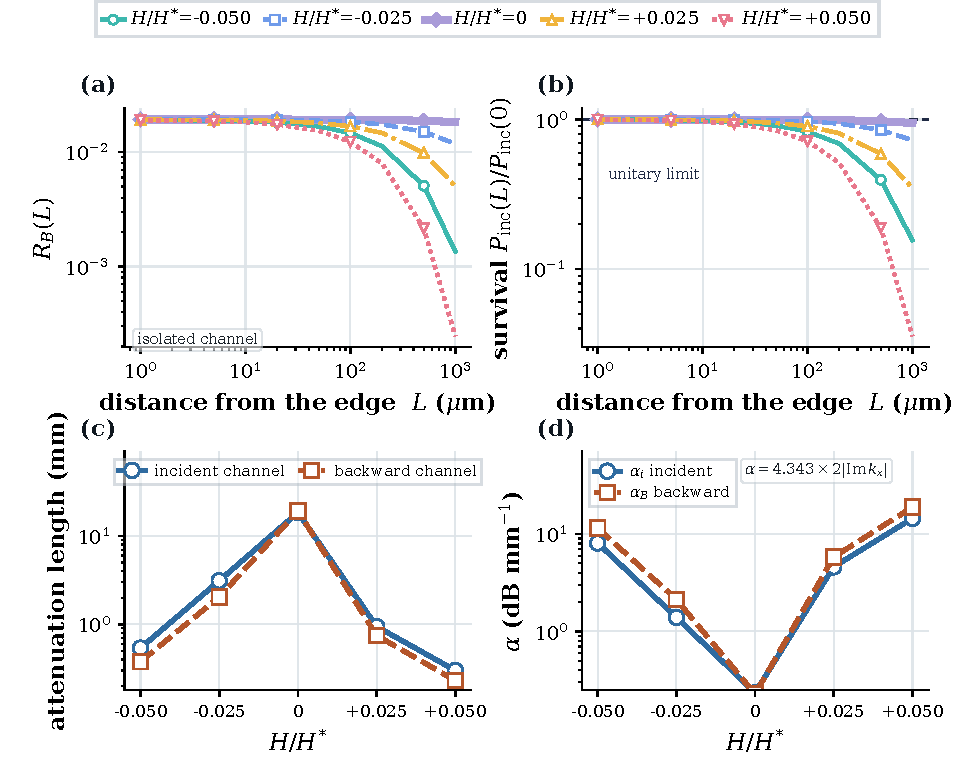
\includegraphics[width=0.95\textwidth]{figures/fig06_attenuation.pdf}
\caption{Distance, survival and attenuation at the operating point. (a) Backward channel against distance from the edge; (b) incident-power survival factor, normalized to its edge value; (c) attenuation length ($1/\alpha$ with $\alpha=2|\Imag k_x|$) and (d) loss coefficient in dB mm$^{-1}$ ($4.343\,\alpha$) against $H/H^{*}$.}
\label{fig:fig06}
\end{figure}

\subsection{Coupling and the through-thickness flux}
\label{sec:results_coupling}
\label{sec:results_boundary}

\Cref{fig:fig07} resolves the two-parameter dependence.  Over the solved box
$0.05\le k_yd\le0.20$ and $-0.05\le H/H^{*}\le0.05$, the backward channel ranges
from $0.01546$ to $0.02180$.  Panel (a) shows that the transverse wavenumber
alone accounts for almost all of that range: the five coupling curves are
displaced but their common slope is set by $k_y$.  Panels (c) and (d) quantify
the displacement: against $H/H^{*}$ at fixed operating frequency the relative
change is at most \SI{2.48}{\percent}, and against $k_y$ it is a slow drift that
never exceeds the same bound.  The ratio of the two sensitivities is the
quantitative statement of this paper about the added coupling: $k_y$ changes the
backward channel by a factor of $1.41$ across the box, while $H$ changes it by
at most \SI{2.5}{\percent} at fixed frequency and by \SI{1.21}{\percent} in the
branch-consistent comparison.  The coupling is a
perturbation of the partition and not its organizing parameter.  The comparison
must be made at fixed $k_x$, because it is the branch and not the coupling that
sets the partition; the two sensitivities do meet, however, at the branch
maximum, where the branch-consistent coupling effect grows to
\SI{36.1}{\percent}.  The $k_y$ sweep of \cref{fig:fig07} was solved at the operating point only.

Panel (b) draws the computed $5\times19$ grid cell by cell, with no
interpolation beyond the computational box and no smoothing between the five
coupling levels.  Every row of the grid satisfies \eqref{eq:admissible}.

\begin{figure}[htbp]
\centering
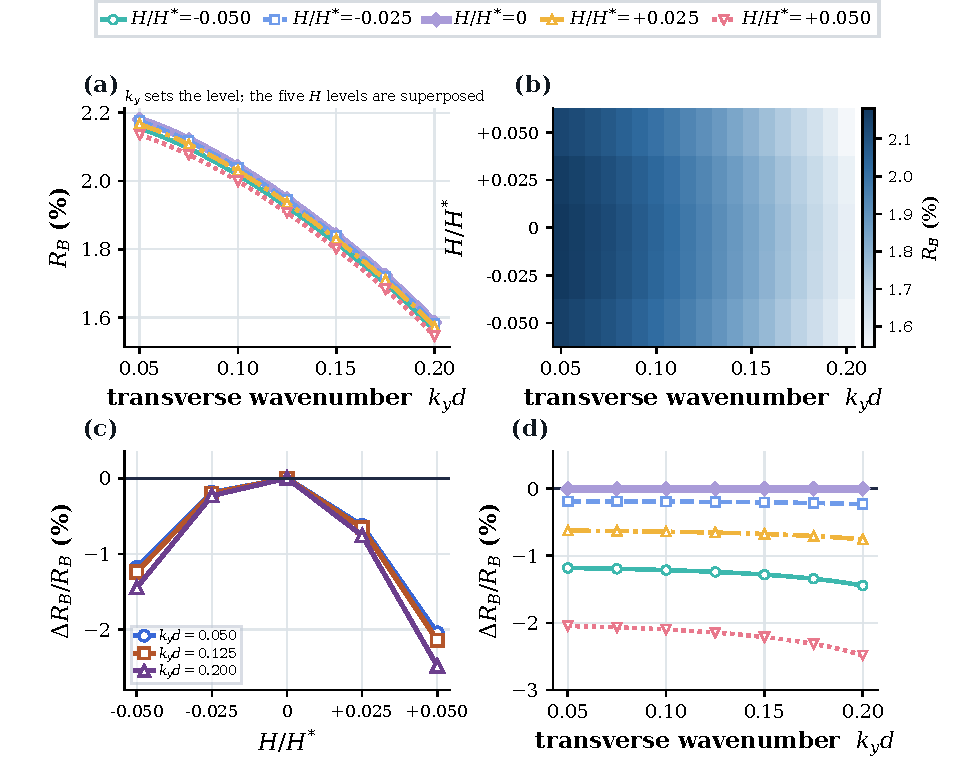
\includegraphics[width=0.95\textwidth]{figures/fig07_coupling.pdf}
\caption{Coupling sensitivity at the operating frequency and wavenumber $k_xd=0.7362$ (the operating point has $k_yd=0.1298$). (a) $R_B$ against $k_yd$ for five $H/H^{*}$; (b) measured $R_B(k_yd,H)$ grid; (c) relative change against $H/H^{*}$ for three $k_yd$; (d) relative change against $k_yd$.}
\label{fig:fig07}
\end{figure}


\Cref{fig:fig08} examines how the backward flux is distributed through the
thickness.  The plotted quantity is the $x$ component of the backward Poynting
flux, normalized by the incident flux, as a function of $z/d$; it is an
evaluated field, not an interpolated surface.

The distribution is a signature of the mode and not of the edge.  The $x$ component
changes sign inside the plate: it is positive near both free surfaces and
negative in the core, reaching $-0.0306$ and $+0.0264$ in units of the thickness-integrated incident flux, while its thickness integral remains negative.  The net backward power is carried by a mode whose local flux direction alternates across the
thickness, which follows from the strain-gradient plate mode itself.  The $z$ component behaves differently: it is largest at the free
surfaces and does not vanish there, so the surfaces carry a transverse flux even
though both traction and double traction vanish on them.  This is the
configuration in which the reactive near field must be retained at the edge
plane, and it explains why the energy budget separates the reactive content from
the transported content instead of adding them.

Panel (c) gives the running thickness integral normalized to its own total, so
the curve rises from zero to one across the plate for each coupling level and
the five curves are indistinguishable.  Panel (d) compares the shape of the
backward and incident $x$ fluxes at $H=0$, both normalized by their own maxima;
both profiles are symmetric about the mid-plane, the incident flux lies mostly near the two faces
(\SI{55}{\percent} of $\int|P_x|\,\dd z$ within $0.1\,d$ of them) and the backward flux does not
(\SI{9}{\percent}).

\begin{figure}[htbp]
\centering
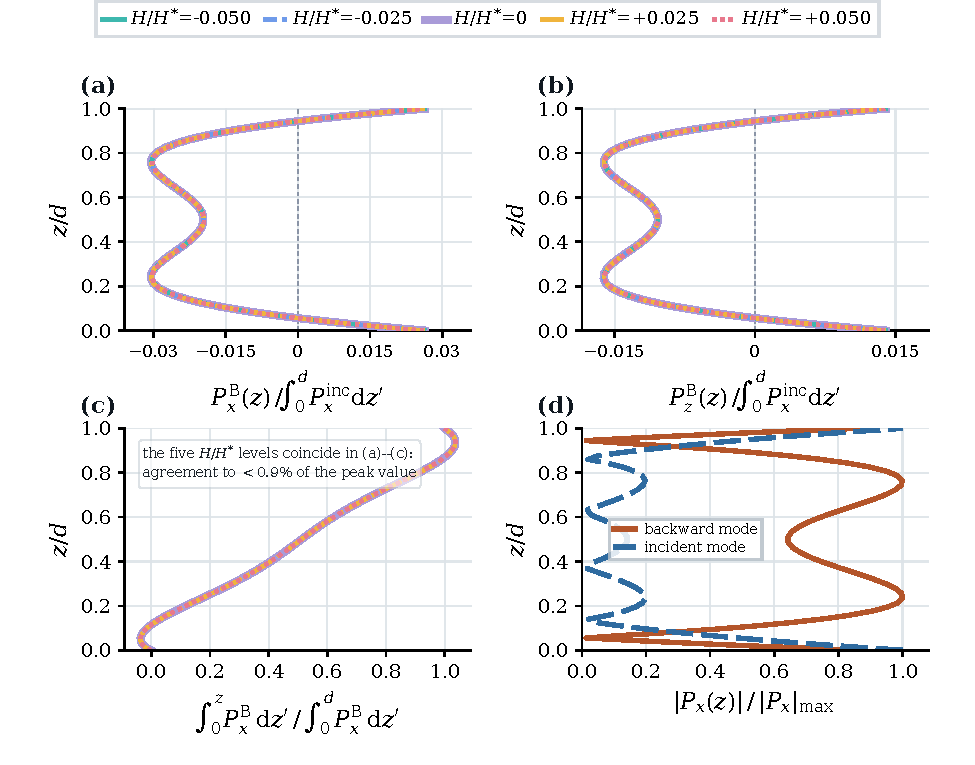
\includegraphics[width=0.95\textwidth]{figures/fig08_boundary.pdf}
\caption{Through-thickness backward flux at the operating point and the reference plane, in units of the thickness-integrated incident flux $\int_0^dP_x^{\mathrm{inc}}\,\dd z$. (a) $P_x^{\mathrm{B}}(z)$ and (b) $P_z^{\mathrm{B}}(z)$ for five $H/H^{*}$; (c) running integral of $P_x^{\mathrm{B}}$; (d) backward and incident $x$ fluxes at $H=0$.}
\label{fig:fig08}
\end{figure}

The coincidence of the five profiles in \cref{fig:fig08}(a)--(c) follows
from the assembly and not from a plotting choice, and it can be quantified.  The coupling enters through the two off-diagonal blocks that connect
the out-of-plane displacement to the carrier, whose entries are
\begin{equation}
\label{eq:H_entry}
\bigl(\mathsf A_{u\mu}\bigr)_{ij}
=h\int_{-1/2}^{1/2}b_i''(s)\,b_j(s)\,\dd s ,
\end{equation}
because $\widetilde\mu$ contains $-h\,\partial_s^{2}u_3$ and \eqref{eq:mu} is
the relation that conveys the coupling; written in the coordinate $\zeta=2s$ of
the field equations the same term acquires a factor four, $4\partial_\zeta^{2}$,
and the measure $\dd s=\dd\zeta/2$ is what keeps \eqref{eq:H_entry} free of it.
Since $b_i''$ has degree $i-2$ and $b_j$ has degree $j$, the matrix of
\eqref{eq:H_entry} vanishes unless $j\le i-2$: it is lower triangular, not upper triangular, and its row norms
$0,\,0,\,26.83,\,91.65,\,222.89,\,450.87,\,809.44$ at degree six grow with the
mode number as the second derivative does, the largest single entry being
$580.5$ in the last row.  With $h=1.06\times10^{-2}$
the largest entry of the assembled block is $6.13$, which is $10.5\%$ of the
inertia scale $\omega^{2}=58.3$ that sets the through-thickness balance of the
lowest rows, and four and a half orders of magnitude below the largest diagonal
entry of the same rows, $2.16\times10^{5}$.  That is a statement about the size of the
coupling, not about a mode: the operator is row-equilibrated before the
eigenvalue problem is formed, so no entry ratio is a frequency.  The size of these entries sets the scale of the coupling in the
assembled operator but is not used to derive the profile differences.  Those are
read from \cref{fig:fig08}(a)--(c): the flux profiles of the five levels differ by
less than \SI{0.9}{\percent} of the peak value, while the partition at the same
coupling changes by \SI{1.21}{\percent} at the operating point.

The same reading applies to the density sweep, where five carrier densities
collapse onto one curve.  The density enters the carrier sector only through the
screening group $Q^{2}=d^{2}q^{2}n_0/(\kappa_{33}k_BT)$, which multiplies the
single potential block $\mathsf A_{\varphi\mu}$, and through the mobility in
$\alpha_{\mathrm d}=\mu_ek_BT/(q\,d\,c_s)$; in the response the two appear as the
conductivity $n_0\mu_e$, so at fixed $n_0\mu_e$ the partition is unchanged and
the collapse reflects that product and not either parameter separately.

The ordering of these sensitivities is a property of the coupling and the operating point together: $k_y$ changes the backward channel by a factor of $1.41$ across the solved box while $H$ moves it by \SI{1.21}{\percent} at the operating point, but at the maximum the coupling moves the partition by \SI{36.1}{\percent}, and the $k_y$ sweep was not repeated there.  Any statement about the added coupling must therefore be made at fixed $k_y$, and an experimental attempt to see it must control the transverse wavenumber much better than the doping or the mobility.

\subsection{Validation and the near field}
\label{sec:results_validation}
\label{sec:results_field}

\Cref{fig:fig09} documents the numerical behavior of the edge solve.  Panels
(a) and (b) show the relative error of the backward channel and of the backward
wavenumber against the degree-33 reference: the channel error falls from
$2.6\times10^{-5}$ at $n=14$ to $1.6\times10^{-6}$ at $n=26$, while the wavenumber error remains at the $10^{-12}$ round-off floor over the full range, so the channel
error is still decreasing at the highest degree shown.  Panel (c)
shows the scaled edge residual and the relative energy-balance error for each degree: the residual is $3\times10^{-15}$, six to seven orders below the
$10^{-8}$ tolerance drawn in the panel, and the energy-balance error lies between $2\times10^{-13}$ and $4\times10^{-12}$, one to three orders below the
$10^{-10}$ line.  Both are round-off in a relative measure, and the panel
shows that neither drifts with the degree.  Panel (d) compares the temporal and spatial routes for the same
dispersion relation across the box; they agree to $2\times10^{-5}$.

The last panel is a check on the implementation, not a physical validation.  The
two routes discretize the same variational statement and differ only in which
variable is used as the eigenvalue; agreement to $2\times10^{-5}$ shows that the
assembly, the boundary conditions and the elimination of the potential are
implemented consistently.

The classical part of the edge solver was compared with the published
free-edge calculation of G\'erardin et al.\ \cite{gerardin2016negative}.  The
ZnO constants were replaced by those of their Duralumin plate ($\rho=\SI{2790}{\kilo\gram\per\cubic\metre}$,
$c_L=\SI{6398}{\metre\per\second}$, $c_T=\SI{3122}{\metre\per\second}$), with no piezoelectricity,
strain gradient or carrier coupling, and the incident $S_1$ mode was taken at normal incidence
($k_y=10^{-7}$ in the units of the solver).  The backward branch appears at
$f\times(2h)=\SI{2.8727}{\mega\hertz\milli\metre}$, against $2.87$ in \cite{gerardin2016negative}.  The
modal share $R_B=|r_{S_1|S_{2b}}|^2$ is $0.9988$ at
\SI{2e-6}{\mega\hertz\milli\metre} above that frequency, which is the
perfect conversion of \cite{gerardin2016negative}, and then falls to $0.797$, $0.500$ and
$0.288$ at $2.90$, $3.00$ and \SI{3.10}{\mega\hertz\milli\metre}, that is $|r|=0.893$, $0.707$ and $0.537$.
Read from their Fig.~2(b) by eye, the corresponding values are about $0.9$, $0.7$ and $0.55$, so the agreement is
within the reading accuracy of the figure; no tabulated values are available for a closer comparison.  Degrees 18 and 26 differ by
less than $10^{-9}$ in $R_B$, the power balance closes to $4\times10^{-11}$ and the edge residual is below $10^{-14}$.  This benchmark covers the classical elastic edge problem only; it does not test the
piezoelectric, strain-gradient or carrier terms.  The independent checks are the strong-form
integrations and the $C^1$ finite-element plate, neither of which shares the spectral matrices
with the production path.

\begin{figure}[htbp]
\centering
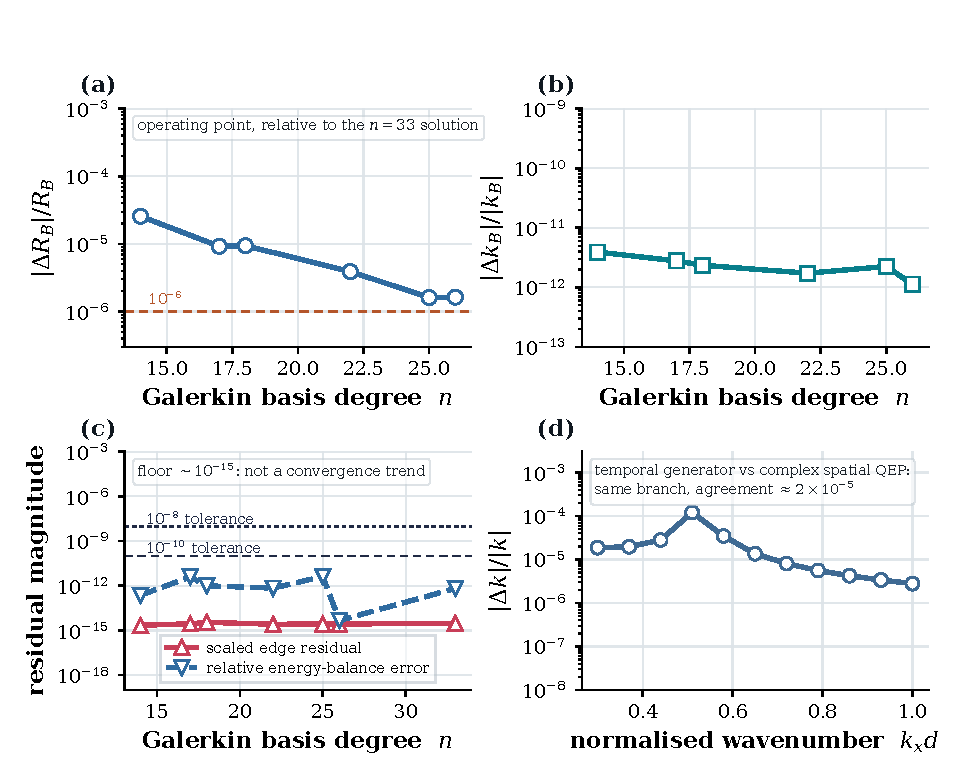
\includegraphics[width=0.95\textwidth]{figures/fig09_validation.pdf}
\caption{Convergence and consistency checks at the operating point. (a) Error of $R_B$ and (b) of the backward wavenumber against the Galerkin degree, relative to the $n=33$ solution; (c) edge residual and energy-balance error; (d) temporal-generator against spatial eigenvalue routes.}
\label{fig:fig09}
\end{figure}


\Cref{fig:fig10} shows the solved field.  Panels (a) and
(b) show the incident and backward intensities on a shared logarithmic color
scale over $x\in[-60,1.5]\,\si{\micro\metre}$ and
$y\in[-45,45]\,\si{\micro\metre}$; the vertical line at $x=0$ is the edge, the
plate lies to its left, and the intensities are normalized to a common maximum
so that the backward field is visibly weaker by one to three decades.  The
incident field approaches the edge at $+10.0^{\circ}$ and the backward field
leaves it at $-27.9^{\circ}$, both measured from the thickness-integrated
Poynting flux and from the $x$ axis along the propagation direction (the $+x$ direction for the incident field, the $-x$ direction for the backward field), positive towards $+y$.

Panel (c) is a schematic, but its arrows are not drawn by hand: they are the
solved directions.  The two wavenumbers point into the plate,
$\vect{k}_i\propto(1,0.176)$ and $\vect{k}_B\propto(1,0.529)$, because $k_y$ is
positive and both axial wavenumbers are real and positive.  The incident flux
follows its wavenumber, $\vect{P}_i\propto(1,0.176)$, whereas the backward flux
is $\vect{P}_B\propto(-1,-0.529)$: the backward mode carries energy in $-x$ and
in $-y$ simultaneously, so its energy transport is opposite in both components
to its own phase direction, and the two flux arrows are the geometric content of
the word ``negative''.  Panel (d) shows the two components of
the backward flux against $k_yd$; both are negative throughout the box, and both
tend to a common small value as $k_yd\to0.2$.

\begin{figure}[htbp]
\centering
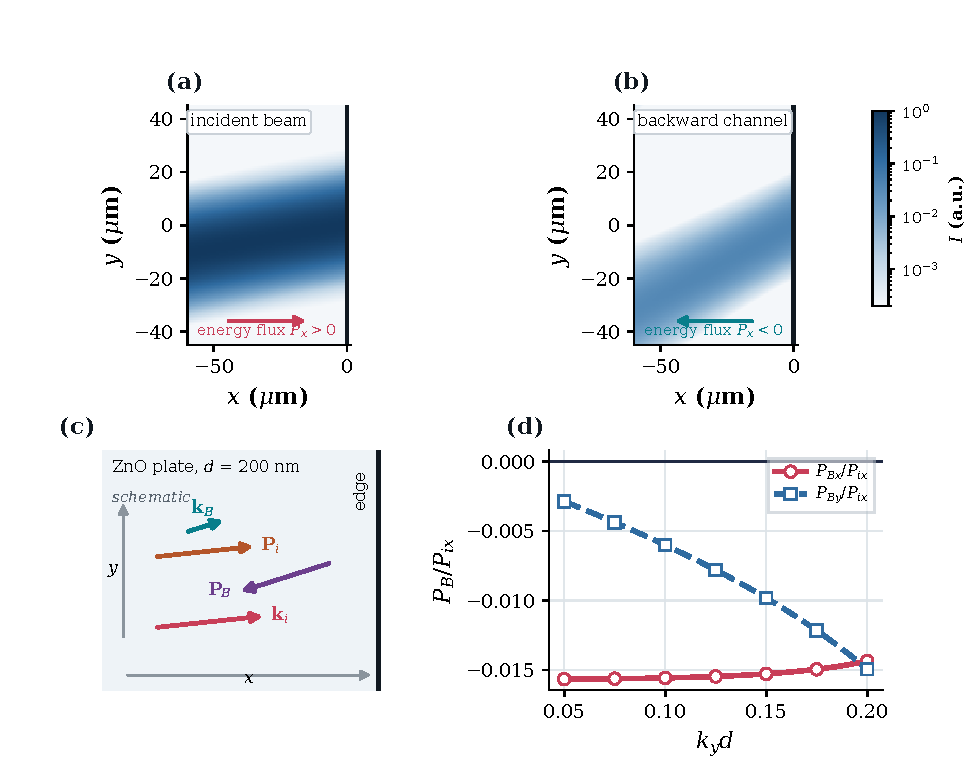
\includegraphics[width=0.95\textwidth]{figures/fig10_field.pdf}
\caption{Field maps and flux directions at the operating point. (a) Incident and (b) backward intensity (arbitrary units, common logarithmic scale) for a Gaussian superposition in $k_yd$ of standard deviation $0.022$ about $0.1298$, edge at $x=0$; (c) schematic of wavenumber and flux directions; (d) components of the backward flux against $k_yd$.}
\label{fig:fig10}
\end{figure}

\subsection{Carrier density and structural loss at the fold}
\label{sec:results_sens}

The two sweeps above vary the carrier density over a factor of three and contain no
loss other than carrier conduction and diffusion.  Because the conversion is largest where the incident
flux nearly vanishes, both limits were tested with the same branch-following definition of $R_B$
($L=10\,d$, $k_yd=0.1298$, $H=0$).

The search for the fold was repeated at six densities from
$2\times10^{18}$ to $2\times10^{23}\,\si{\per\cubic\metre}$, which takes $Q=d/L_D$ from $0.075$ to $24$.  This range covers the densities of nominally undoped ZnO compiled in Table~VII of \cite{ozgur2005zno}, $8\times10^{19}$--$5\times10^{23}\,\si{\per\cubic\metre}$, up to its upper end.  The
maximum falls from $0.943$ through $0.828$ to $0.545$ over the first three densities ($2\times10^{18}$, $2\times10^{19}$, $2\times10^{20}\,\si{\per\cubic\metre}$), with the argmax inside the raster.  From
$2\times10^{21}\,\si{\per\cubic\metre}$ upward the largest sampled value in a window of $\pm0.03$ about the
fold lies on the edge of the window, so the entries ($\ge0.168$, $\ge0.043$ and $\ge0.174$) are lower bounds and the maximum itself was not located.  At the operating
point, which was swept over a wider range than the fold search, the share stays between $0.0158$ and $0.0410$ over the whole range $2\times10^{18}$ to
$6\times10^{23}\,\si{\per\cubic\metre}$, and its linewidth peaks near $2\times10^{22}\,\si{\per\cubic\metre}$ at
\SI{8.7}{\mega\hertz}.  The statement of \cref{sec:results_material} that the density sets the loss but not the
partition therefore holds for the range of \cref{fig:fig02}; at the fold the partition depends on the density through the loss.


For orientation, Zhang et al.\ \cite{zhang2025pscplate} find for a simply supported plate under static load and in free vibration that the semiconductor coupling is active only within a window of initial electron concentration, which moves to larger concentrations as the plate becomes thinner; the concentration at which their damping is largest is $10^{18.6}$, $10^{19.6}$ and $10^{20.6}\,\si{\per\cubic\metre}$ for $h=30$, $3$ and $0.3\,\si{\micro\metre}$.  The present plate ($d=\SI{200}{\nano\metre}$, $n_0\le3\times10^{18}\,\si{\per\cubic\metre}$ in the main sweeps) lies below these values, so the carrier results describe the weakly conducting side of that window.  For shear-horizontal waves in ZnO plates, Li et al.\ \cite{li2023sh} report that an initial density below $2\times10^{18}\,\si{\per\cubic\metre}$ barely changes the cut-off frequencies and that above $10^{23}\,\si{\per\cubic\metre}$ the plate responds as an elastic one, which is consistent with the density range scanned here.  Dispersion and damping of Rayleigh-type waves in a piezo-thermo-electric semiconductor with fractional and nonlocal effects have also been computed \cite{aldandani2026kg}.


The model contains no intrinsic elastic loss.  To measure the effect of one, the elastic
and gradient-elastic tensors were multiplied by $1-\mathrm i\eta$ (time dependence $e^{-\mathrm i\omega t}$), a loss tangent $\eta$, i.e.\ a
quality factor $1/\eta$, with the carrier terms unchanged.  The form and the values of $\eta$ are assumed; none is taken from a measurement.  Viscoelastic loss of the Kelvin--Voigt type has been treated for nonlocal piezo-semiconductors elsewhere \cite{gupta2026heatmap}.
The frequency was scanned over 41 values within $\pm3\times10^{-3}$ of the lossless fold frequency and the largest $R_B$ is
reported, so that each entry is a lower bound on the maximum over frequency.  Refining the scan around its largest value in four successive steps, down to a window of $7.5\times10^{-7}$ in relative frequency, changes the entries to $0.6003$ and $0.1967$, so the figures quoted below are converged in frequency.  The scan shows that $\eta=10^{-5}$
lowers the maximum from $0.943$ to $0.600$ and $\eta=10^{-4}$ to $0.197$, while
$|\Imag k_{ix}|d$ rises from $1.0\times10^{-3}$ to $8.1\times10^{-3}$ and $2.0\times10^{-2}$.  This is the square-root response of the
spatial roots to a small loss near a zero-group-velocity point.  For $\eta\ge10^{-3}$ the port selection finds no
propagating incident mode in the scan window and the entries are not evaluated.  The value
$0.943$ is therefore that of a plate whose only loss is carrier conduction, and it should be read as an upper bound
for a real plate.

